\chapter{\ifproject%
\ifenglish Project Structure and Methodology\else โครงสร้างและขั้นตอนการทำงาน\fi
\else%
\ifenglish Project Structure\else โครงสร้างของโครงงาน\fi
\fi
}

ในบทนี้จะกล่าวถึงหลักการ และการออกแบบระบบ

\section{อุปกรณ์ตรวจวัดความหนาแน่น}
\subsection{โครงสร้างของอุปกรณ์}
\begin{figure}[h!]
  \begin{center}
    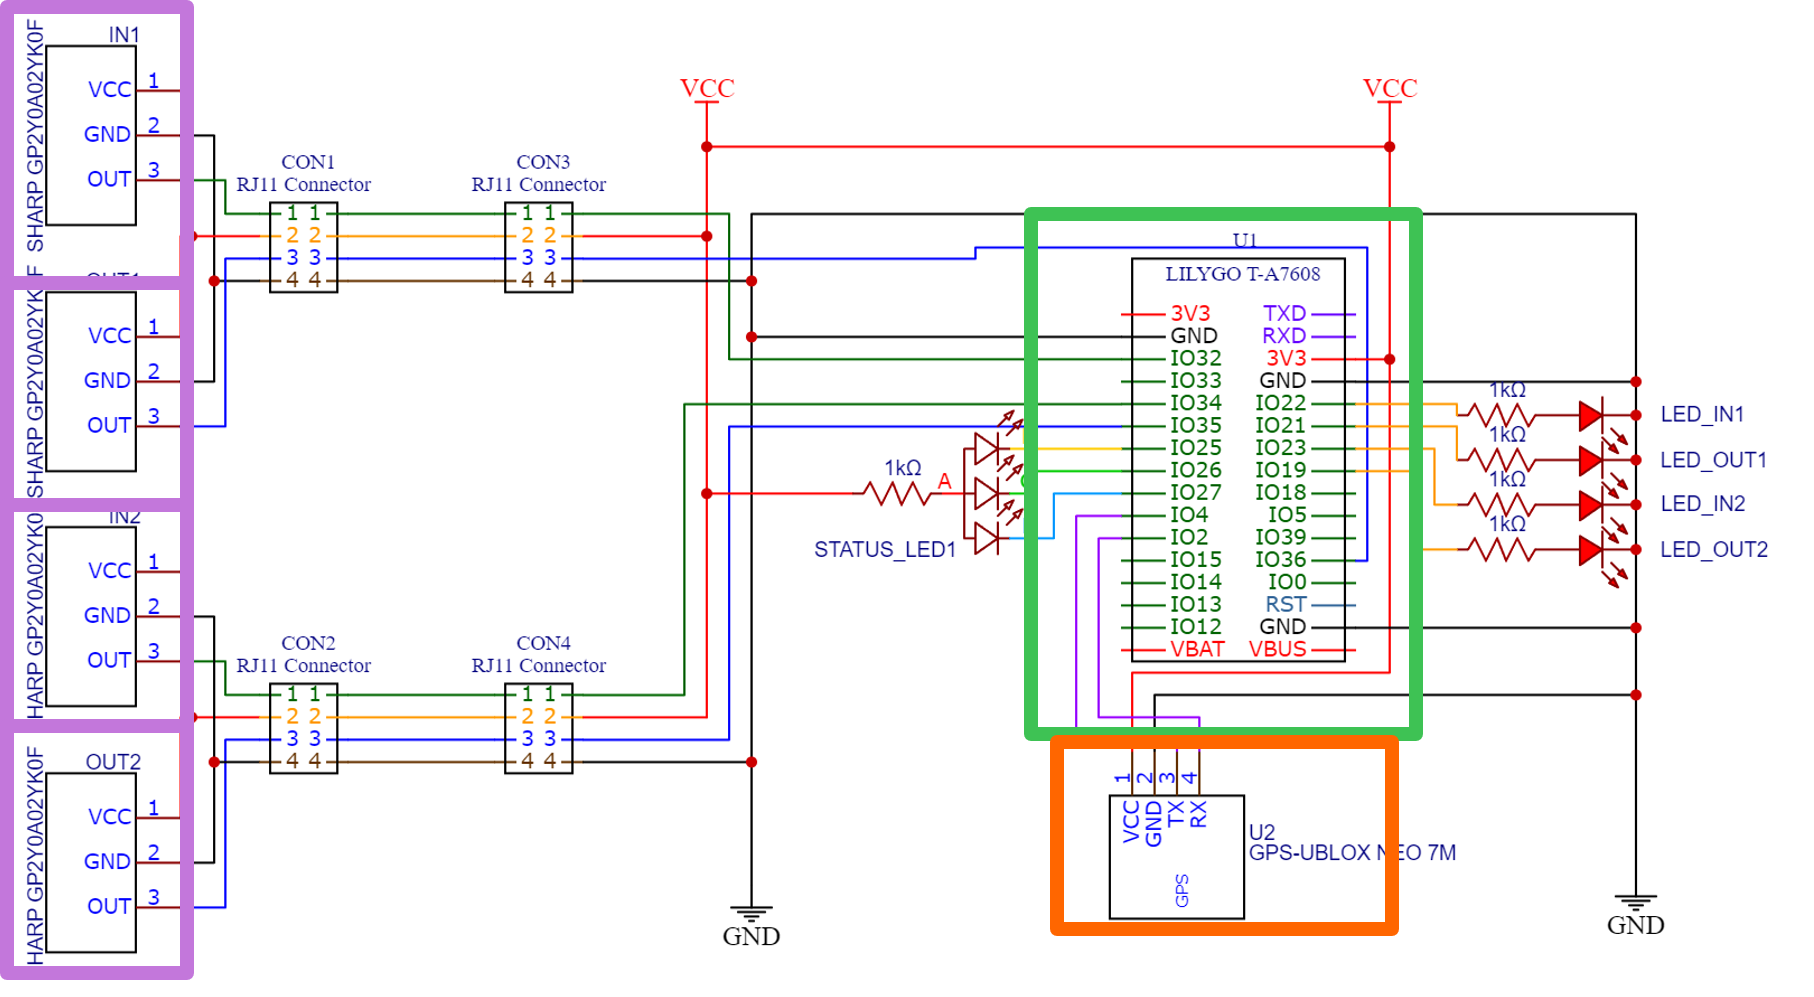
\includegraphics[width=1\textwidth]{schematic-framed.png}
  \end{center}
  \caption{โครงสร้างวงจรของอุปกรณ์}
  \label{fig:schematic-framed}
\end{figure}

อุปกรณ์จะประกอบไปด้วย
\begin{itemize}
  \item บอร์ดสำหรับพัฒนา LILYGO T-A7608 (สีเขียวดังภาพที่ \ref{fig:schematic-framed}) สำหรับประมวลผลข้อมูลที่ได้จากอุปกรณ์วัดต่างๆ และรับ-ส่งข้อมูลกับระบบเชื่อมต่อและแสดงผลข้อมูล
  \item อุปกรณ์รับ-ส่งข้อมูล GNSS u-blox Neo-7M (สีส้มดังภาพที่ \ref{fig:schematic-framed}) สำหรับ รับ-ส่งค่าตำแหน่งของอุปกรณ์
  \item อุปกรณ์วัดระยะห่างโดยใช้อินฟราเรด Sharp GP2Y0A02YK0F 4 ชิ้น โดยติดประคูละ 2 ชิ้น ใกล้กันในแนวระนาบ สำหรับวัดการ เข้า-ออก ของผู้โดยสาร
\end{itemize}

\begin{figure}[h!]
  \begin{center}
    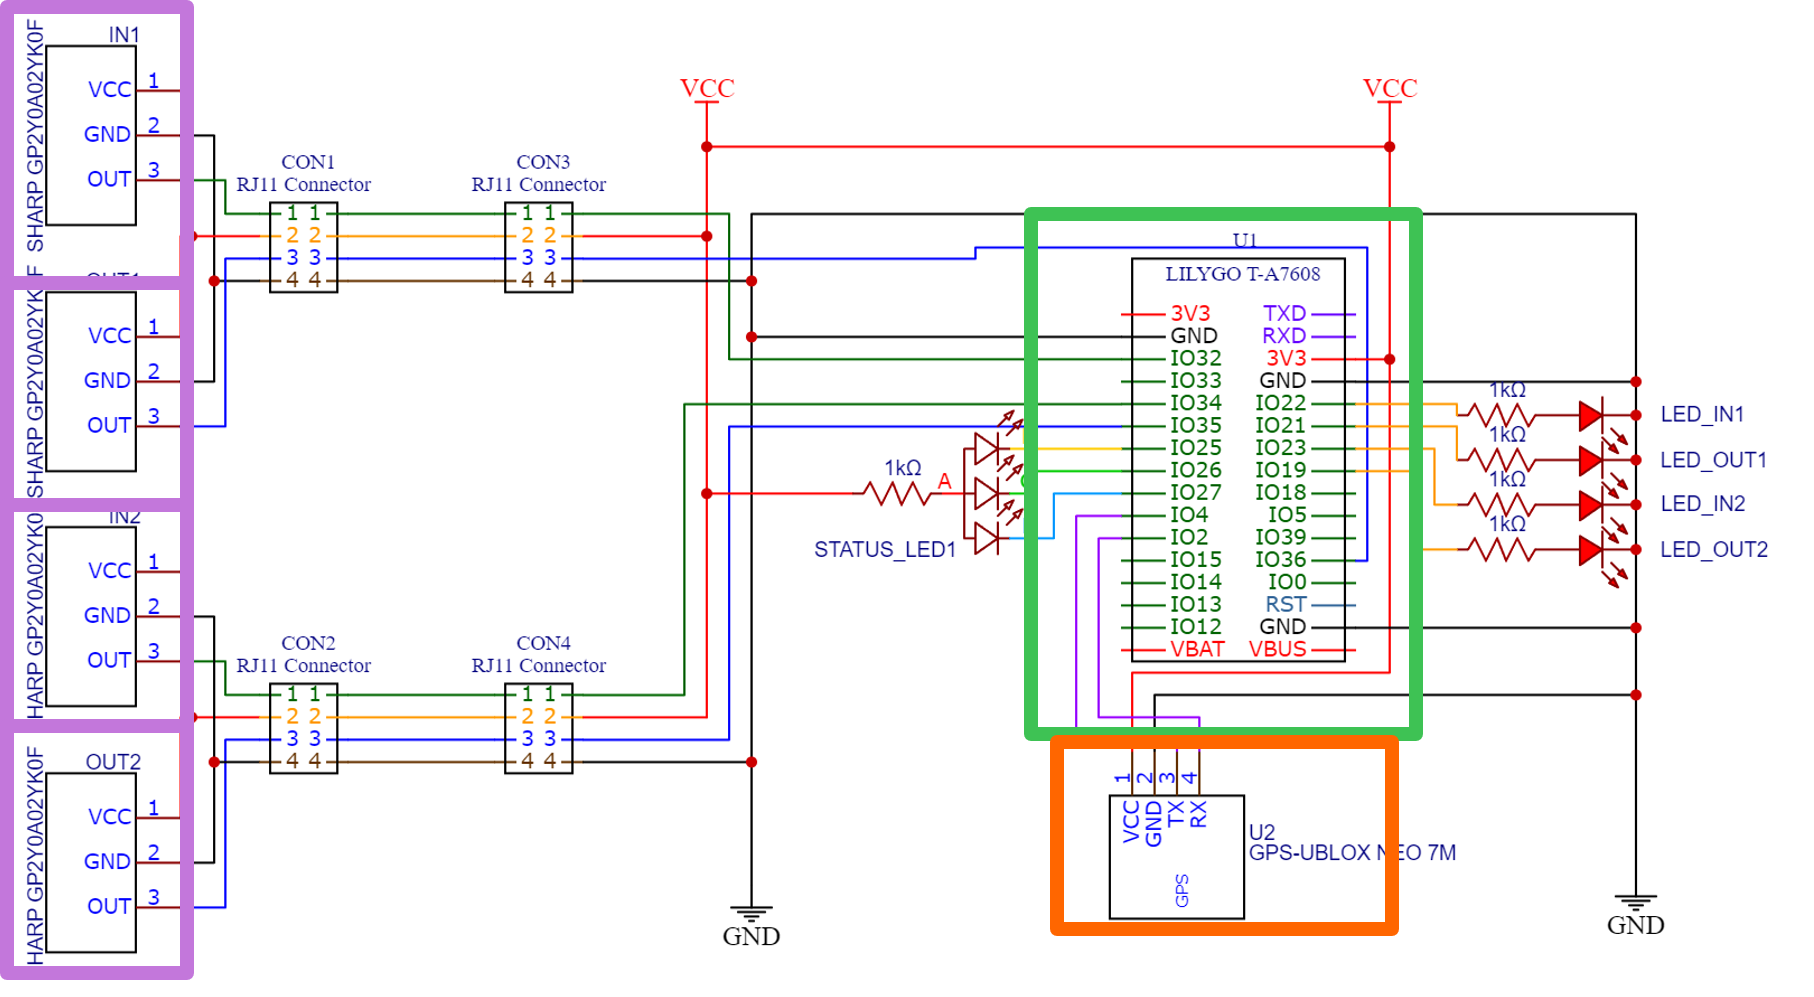
\includegraphics[width=0.75\textwidth]{schematic-framed.png}
  \end{center}
  \caption[อุปกรณ์วัดต้นแบบ]{อุปกรณ์วัดต้นแบบ (บอร์ดพัฒนาและอุปกรณ์รับ-ส่งข้อมูล GNSS อยู่ที่กล่องกลาง ส่วนอุปกรณ์วัดระยะห่างโดยใช้อินฟราเรด อยู่ที่กล่องซ้ายและขวา)}
  \label{fig:schematic-framed}
\end{figure}

\subsection{การทํางานของอุปกรณ์ตรวจวัด}

\begin{figure}[h!]
  \begin{center}
    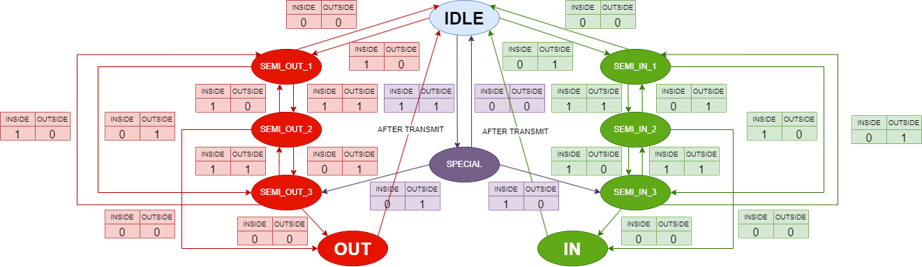
\includegraphics[width=1\textwidth]{state-machine.png}
  \end{center}
  \caption{State Machine ของอุปกรณ์วัด}
  \label{fig:state-machine}
\end{figure}


\subsection{การทํางานของอุปกรณ์ตรวจวัด}

อุปกรณ์จะวัดความหนาแน่นโดยดูจากการเข้า-ออกของผู้โดยที่ประตูผู้โดยสารที่ประตูผู้โดยสารดัง State Matchine ที่\ref{fig:state-machine} โดยหากมีวัตถุอยู่หน้าอุปกรณ์วัดระยะห่างน้อยกว่าที่กำหนด จะนับว่าอุปกรณ์วัดนั้นมีค่าเป็น 1 และเป็น 0 ในทางตรงกันข้าม สำหรับอุปกรณ์วัดการเข้าออกจะเป็น 2 ชุด แต่ละชุดจะมี INSIDE สำหรับอุปกรณ์ฝั่งใกล้ห้องผู้โดยสาร และ OUTSIDE สำหรับอุปกรณ์ฝั่งใกล้ประตู และจะส่งข้อมูลของแต่ละชุดไปยังอุปกรณ์พัฒนาเพื่อประมวลผลข้อมูล ที่มีสถานะดังนี้

\begin{itemize}
  \item IDLE : สถานะเริ่มต้น
  \item SEMI\_OUT\_1: อุปกรณ์วัดระยะห่าง INSIDE ตรวจพบวัตถุก่อน
  \item SEMI\_OUT\_2: อุปกรณ์วัดระยะห่าง INSIDE และ OUTSIDE ตรวจพบวัตถุกพร้อมกันหลัง SEMI\_OUT\_1
  \item SEMI\_OUT\_3: อุปกรณ์วัดระยะห่าง OUTSIDE ตรวจพบวัตถุหลังอุปกรณ์วัดระยะห่าง INSIDE ไม่ตรวจพบวัตถุ
  \item OUT: ผู้โดยสารออกจากรถโดยสาร (นับผู้โดยสารลดลง 1)
  \item SEMI\_IN\_1: อุปกรณ์วัดระยะห่าง OUTSIDE ตรวจพบวัตถุก่อน
  \item SEMI\_IN\_2: อุปกรณ์วัดระยะห่าง INSIDE และ OUTSIDE ตรวจพบวัตถุกพร้อมกันหลัง SEMI\_IN\_1
  \item SEMI\_IN\_3: อุปกรณ์วัดระยะห่าง INSIDE ตรวจพบวัตถุหลังอุปกรณ์วัดระยะห่าง OUTSIDE ไม่ตรวจพบวัตถุ
  \item IN: ผู้โดยสารเข้าสู่รถโดยสาร (นับผู้โดยสารเพิ่มขึ้น 1)
  \item SPECIAL: อุปกรณ์วัดระยะห่าง INSIDE และ OUTSIDE ตรวจพบวัตถุกพร้อมกันหลัง IDLE
\end{itemize}



\subsection{การส่งข้อมูล}

\begin{figure}[h!]
  \begin{center}
    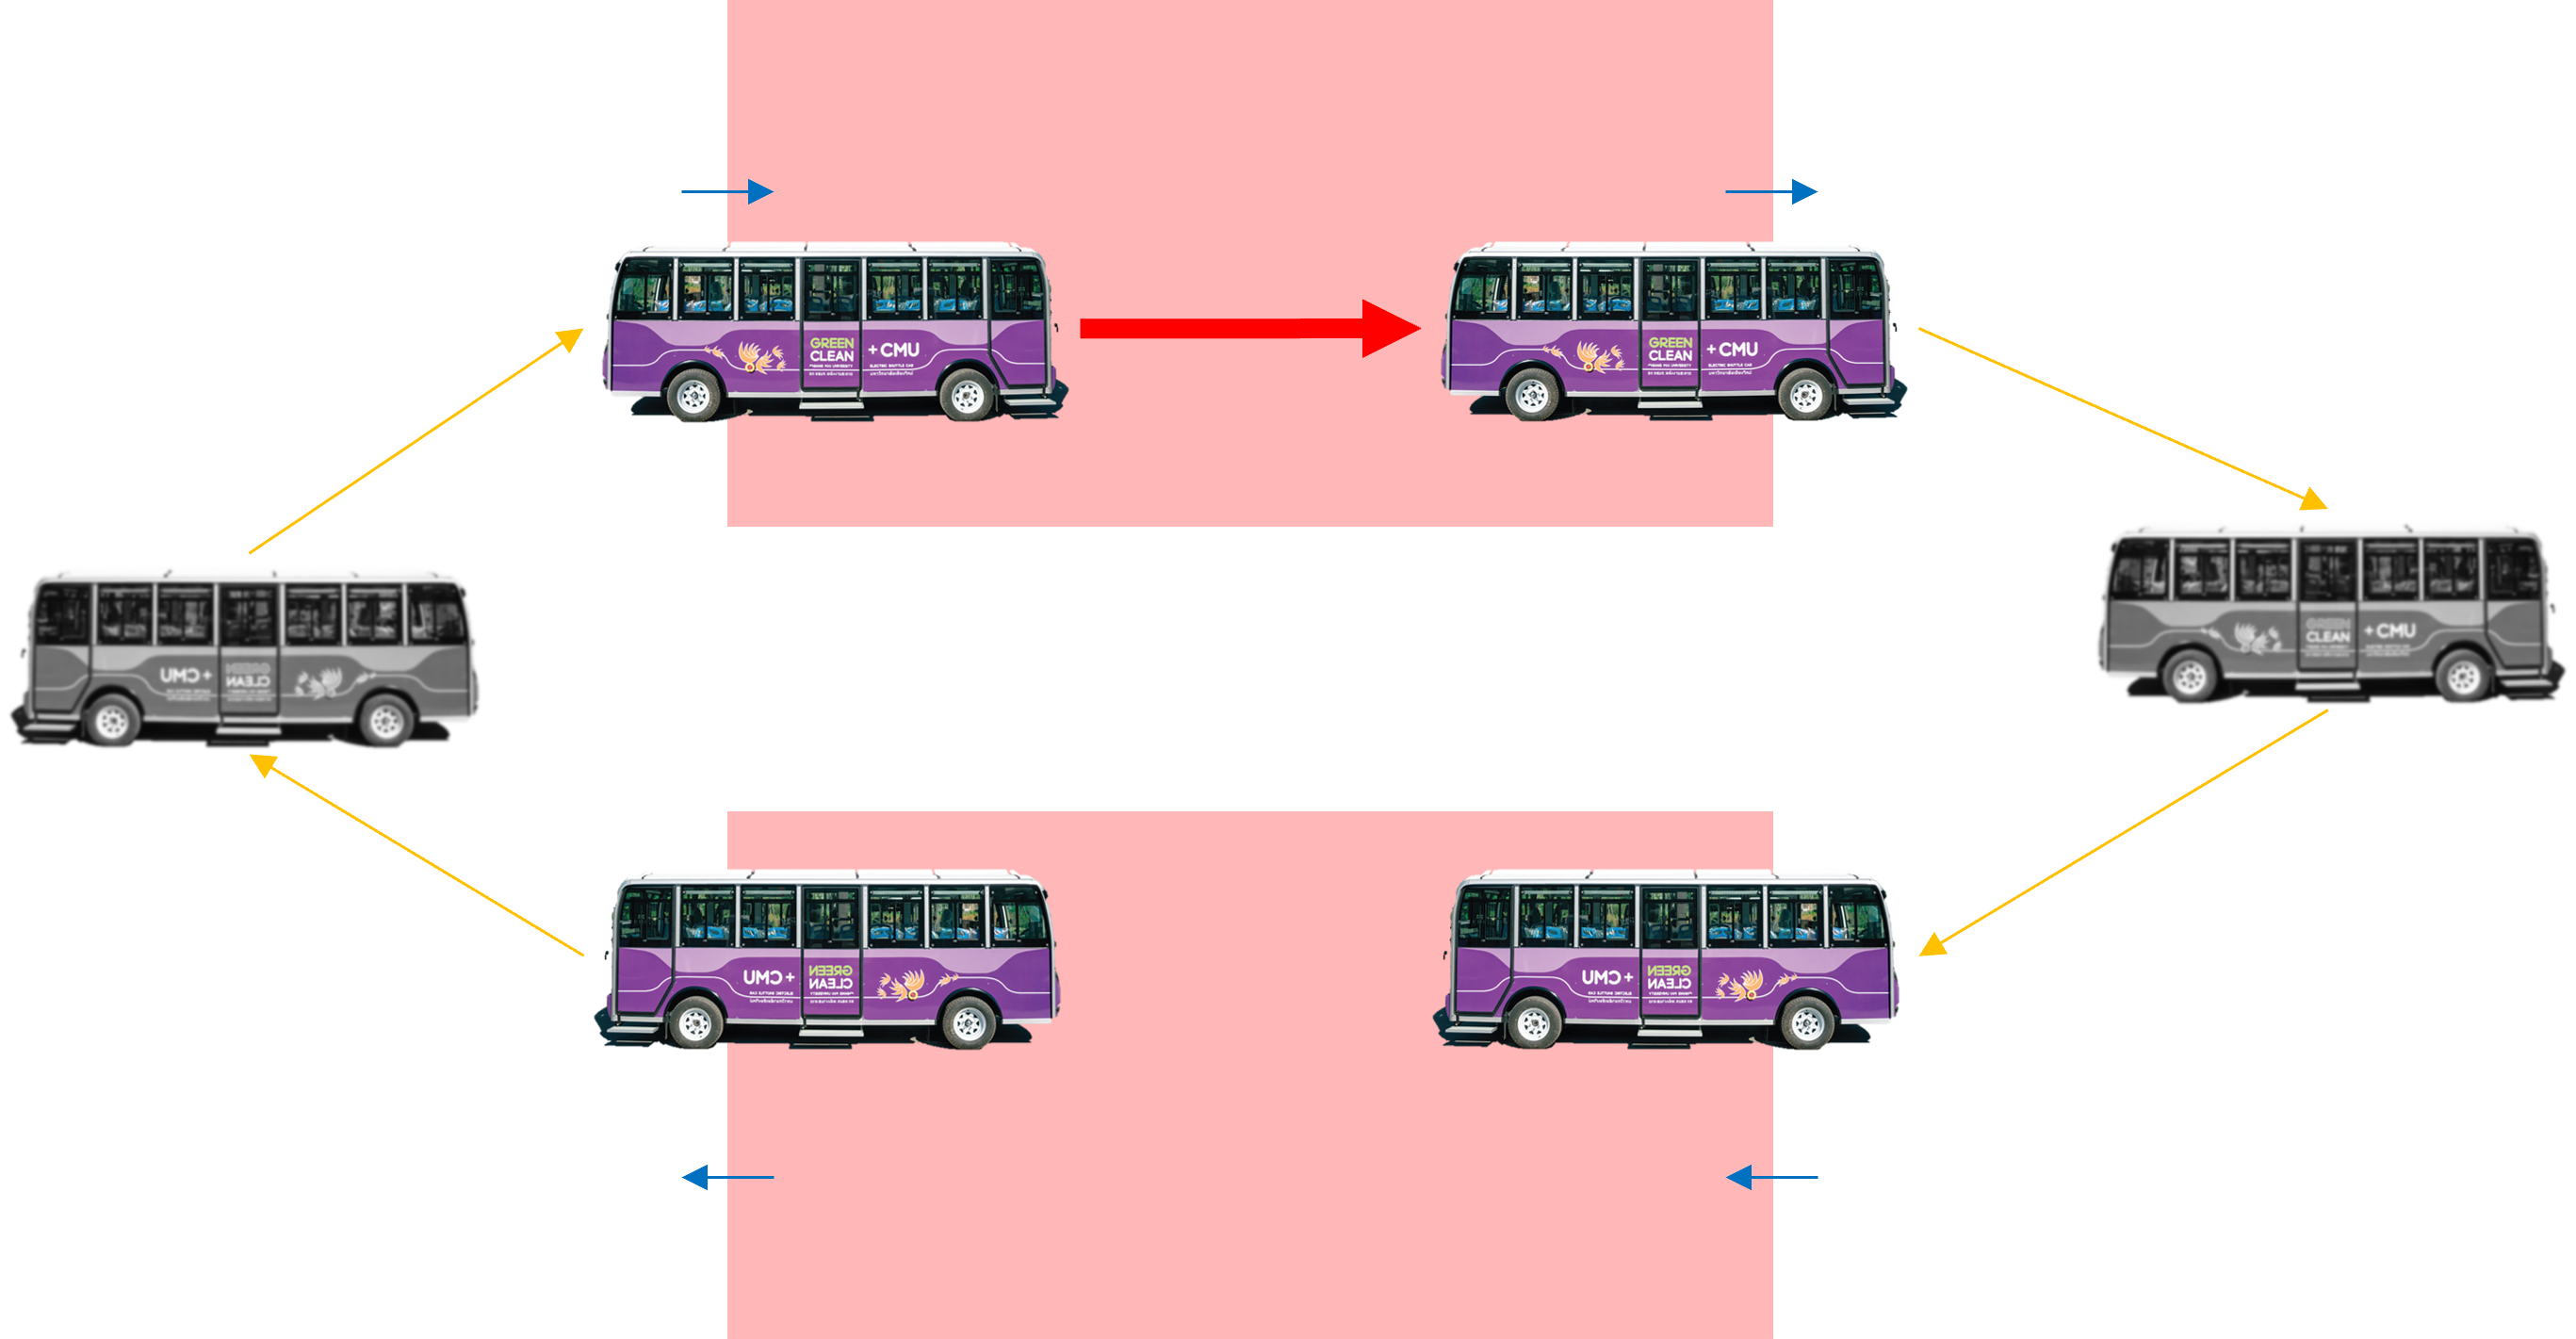
\includegraphics[width=1\textwidth]{msg-transmit.png}
  \end{center}
  \caption{การส่งข้อมูล}
  \label{fig:msg-transmit}
\end{figure}

อุปกรณ์จะรับข้อมูลพื้นที่สถานีจากระบบเชื่อมต่อและแสดงผลข้อมูล และส่งข้อมูลของตัวเองไปยังระบบเชื่อมต่อและแสดงผลข้อมูล (ลูกศรสีน้ำเงินดังภาพที่ \ref{fig:msg-transmit}) โดยใช้ระบบ MQTT เมื่อรถโดยสารเข้าสู้สถานีและออกจากสถานี(กรอบสีแดงดังภาพที่ \ref{fig:msg-transmit}) รวมไปถึงหากไม่เข้า - ออกสถานีเกิน 5 นาที ก็จะส่งข้อมูลเช่นกัน การตรวจวัดความหนาแน่นจะเกิดขึ้นเมื่อรถโดยสารอยู่ในเขตสถานีเท่านั้น

\subsection{รูปแบบการส่งข้อมูล}

\begin{figure}[h!]
  \begin{center}
    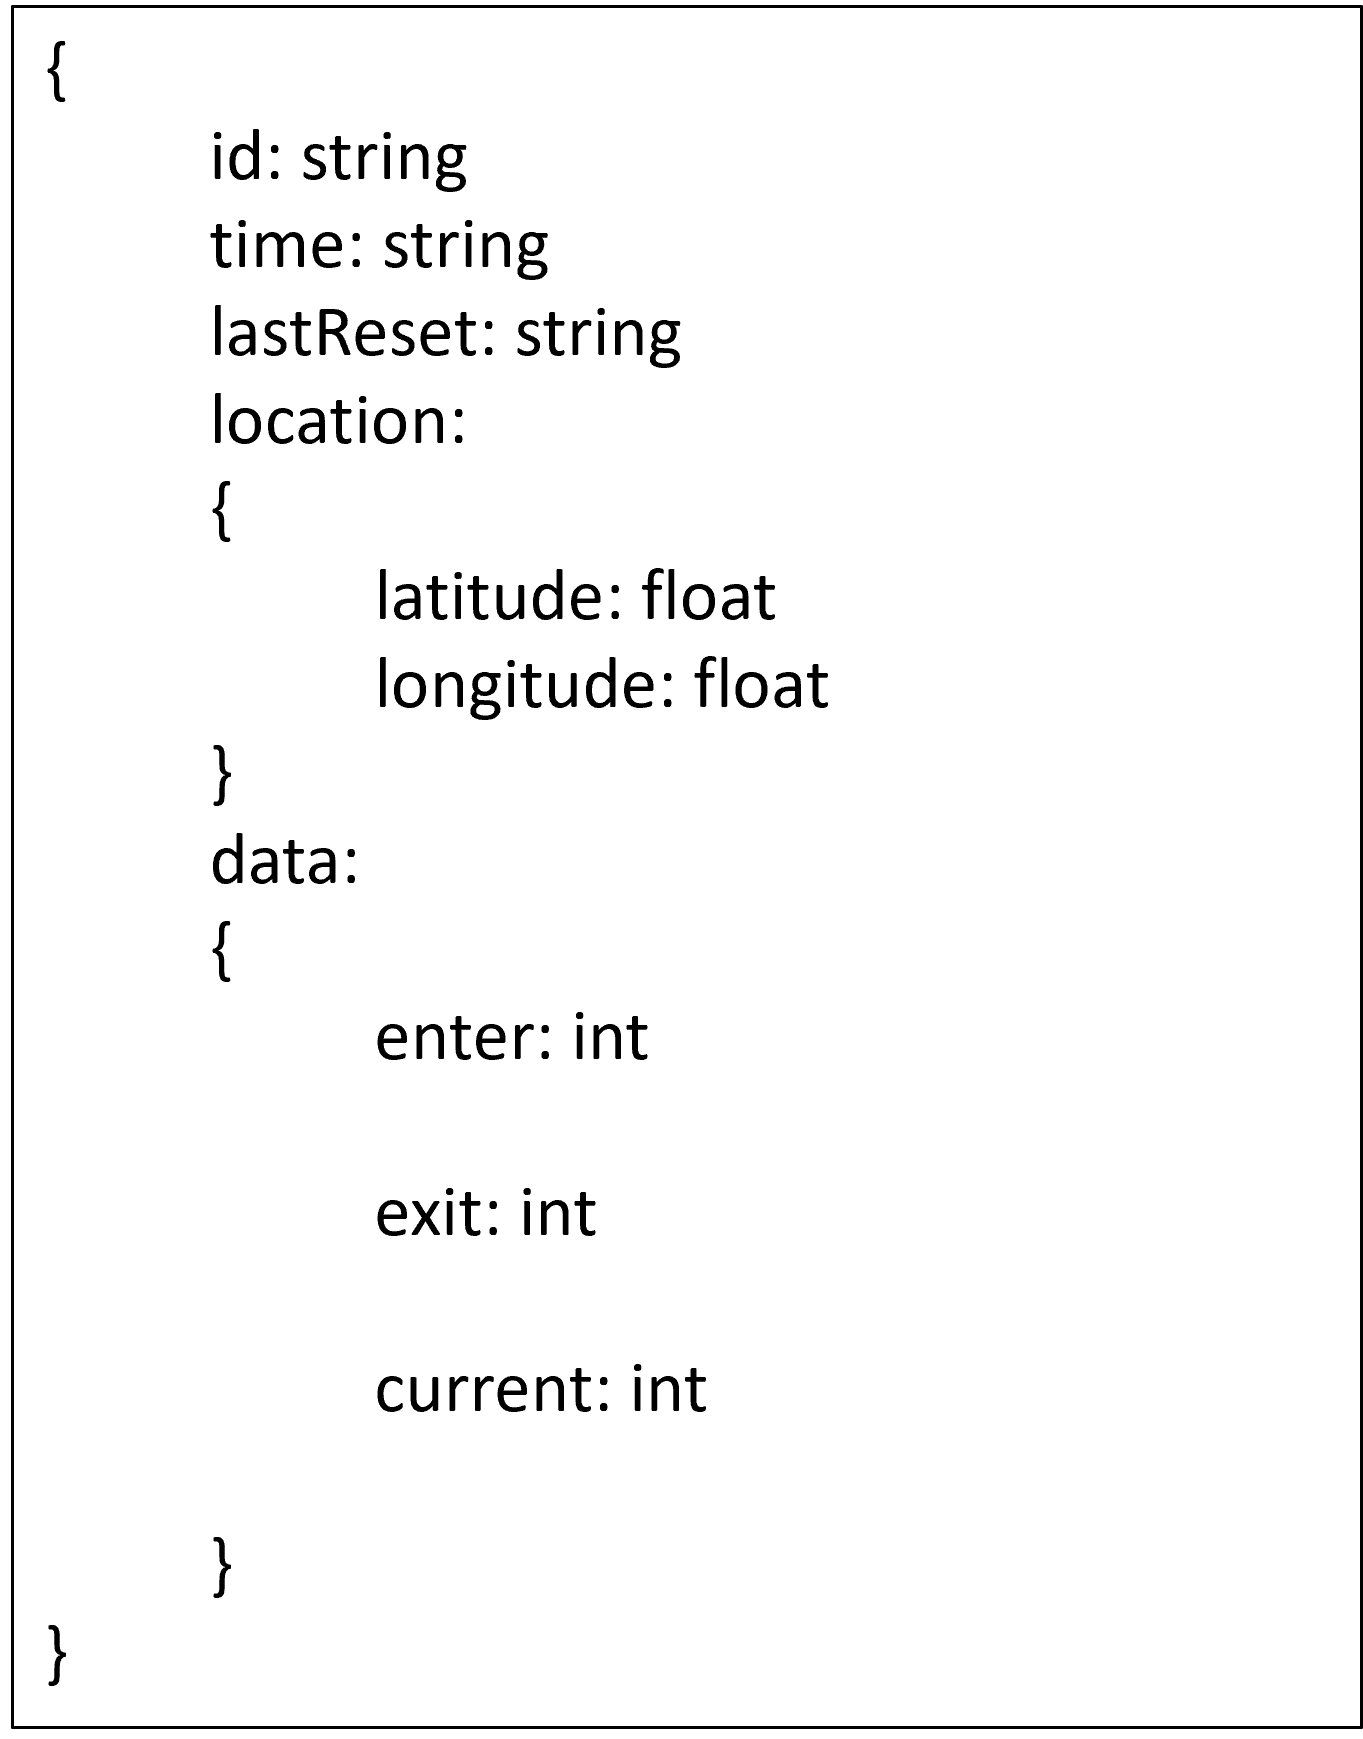
\includegraphics[width=0.5\textwidth]{data-schema.png}
  \end{center}
  \caption{รูปแบบการส่งข้อมูล}
  \label{fig:data-schema}
\end{figure}

อุปกรณ์จะส่งข้อมูลภาพรวมของความหนาแน่นทุกครั้งที่เข้า/ออกสถานี ดังนี้
\begin{itemize}
  \item หมายเลขอุปกรณ์
  \item เวลาที่เข้า/ออกสถานี
  \item เวลาที่รีเซ็ตข้อมูล (โดยปกติจะเป็นเวลาเที่ยงคืน และ เวลาเปิดเครื่อง)
  \item ตำแหน่งของอุปกรณ์
  \item ข้อมูลความหนาแน่น (จำนวนคนเข้า/ออก จำนวนคนบนรถในปัจจุบัน)
\end{itemize}

\subsection{ระบบเชื่อมต่อและแสดงผลข้อมูล}

\subsection{การเชื่อมต่อ (Back-end)}
จะรับข้อมูลมาจากอุปกรณ์ IoT โดยใช้ระบบ MQTT และนำมาประมวลผลโดยใช้ Node.js และนำข้อมูลส่งไปที่การแสดงผลโดยใช้ API ของ Express เพื่อนำข้อมูลส่งขึ้นไปการแสดงผล และนำข้อมูลไปเก็บไว้ใน Database ของ Influxdb

\begin{figure}[h!]
    \begin{center}
      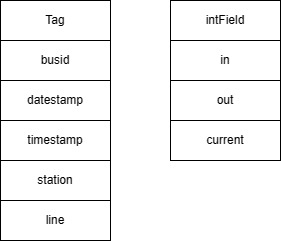
\includegraphics[width=0.75\textwidth]{dbschema.jpg}
    \end{center}
    \caption[Poem]{Database Schema}
    \label{fig:dbschema}
  \end{figure}

\subsection{การแสดงผลข้อมูล (Front-end)}
รับข้อมูลจาก Back-end จากการ Fetch ข้อมูลที่ส่งมาจาก API และนำมาแสดงผลโดยใช้ React.js โดยสามารถเข้าถึงข้อมูลปัจจุบัน และสามารถเข้าถึงข้อมูลในอดีตได้

\begin{figure}[h!]
    \begin{center}
      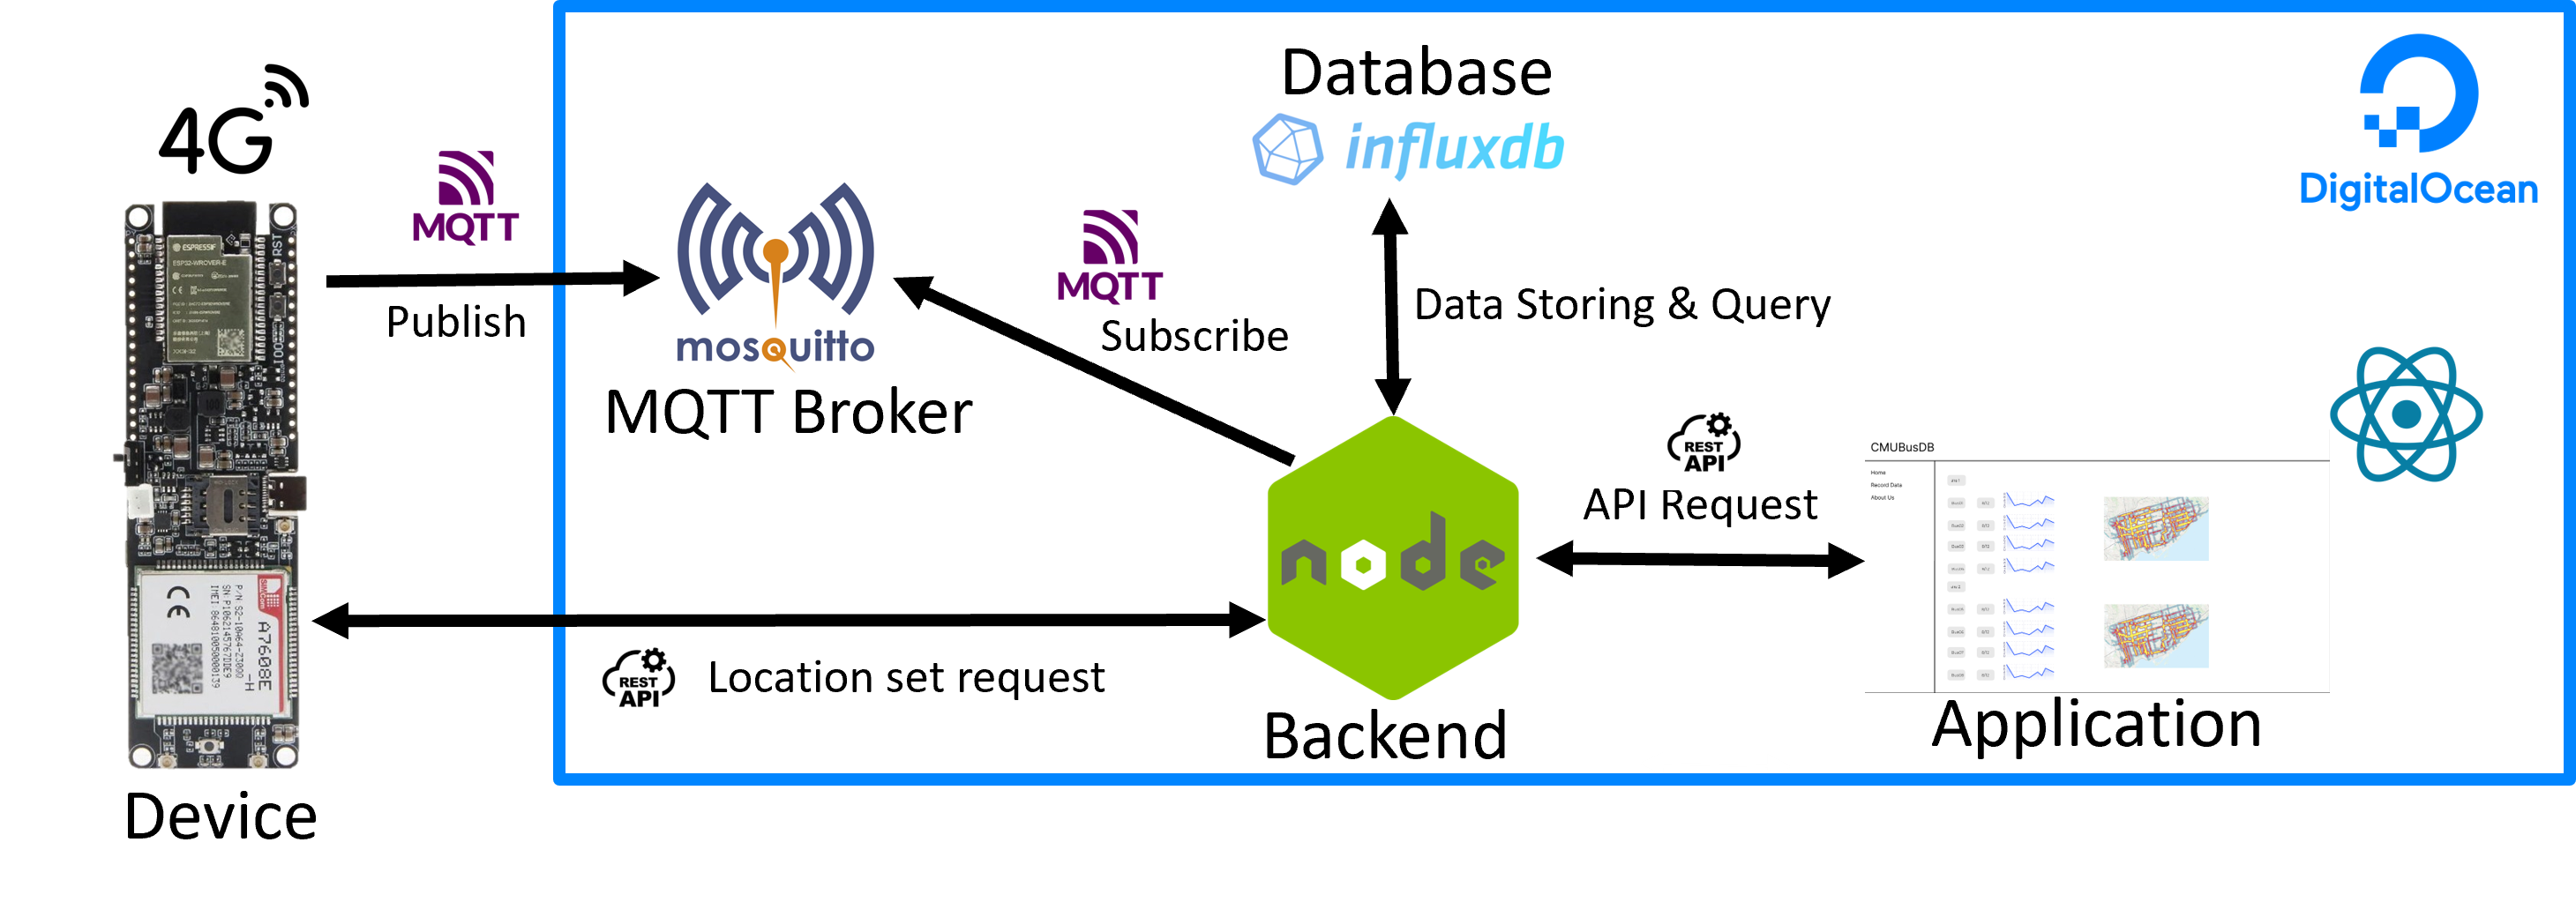
\includegraphics[width=0.75\textwidth]{exchange-data.png}
    \end{center}
    \caption{การแลกเปลี่ยนข้อมูล}
    \label{fig:exchangedata}
  \end{figure}

  \begin{figure}[h!]
    \begin{center}
      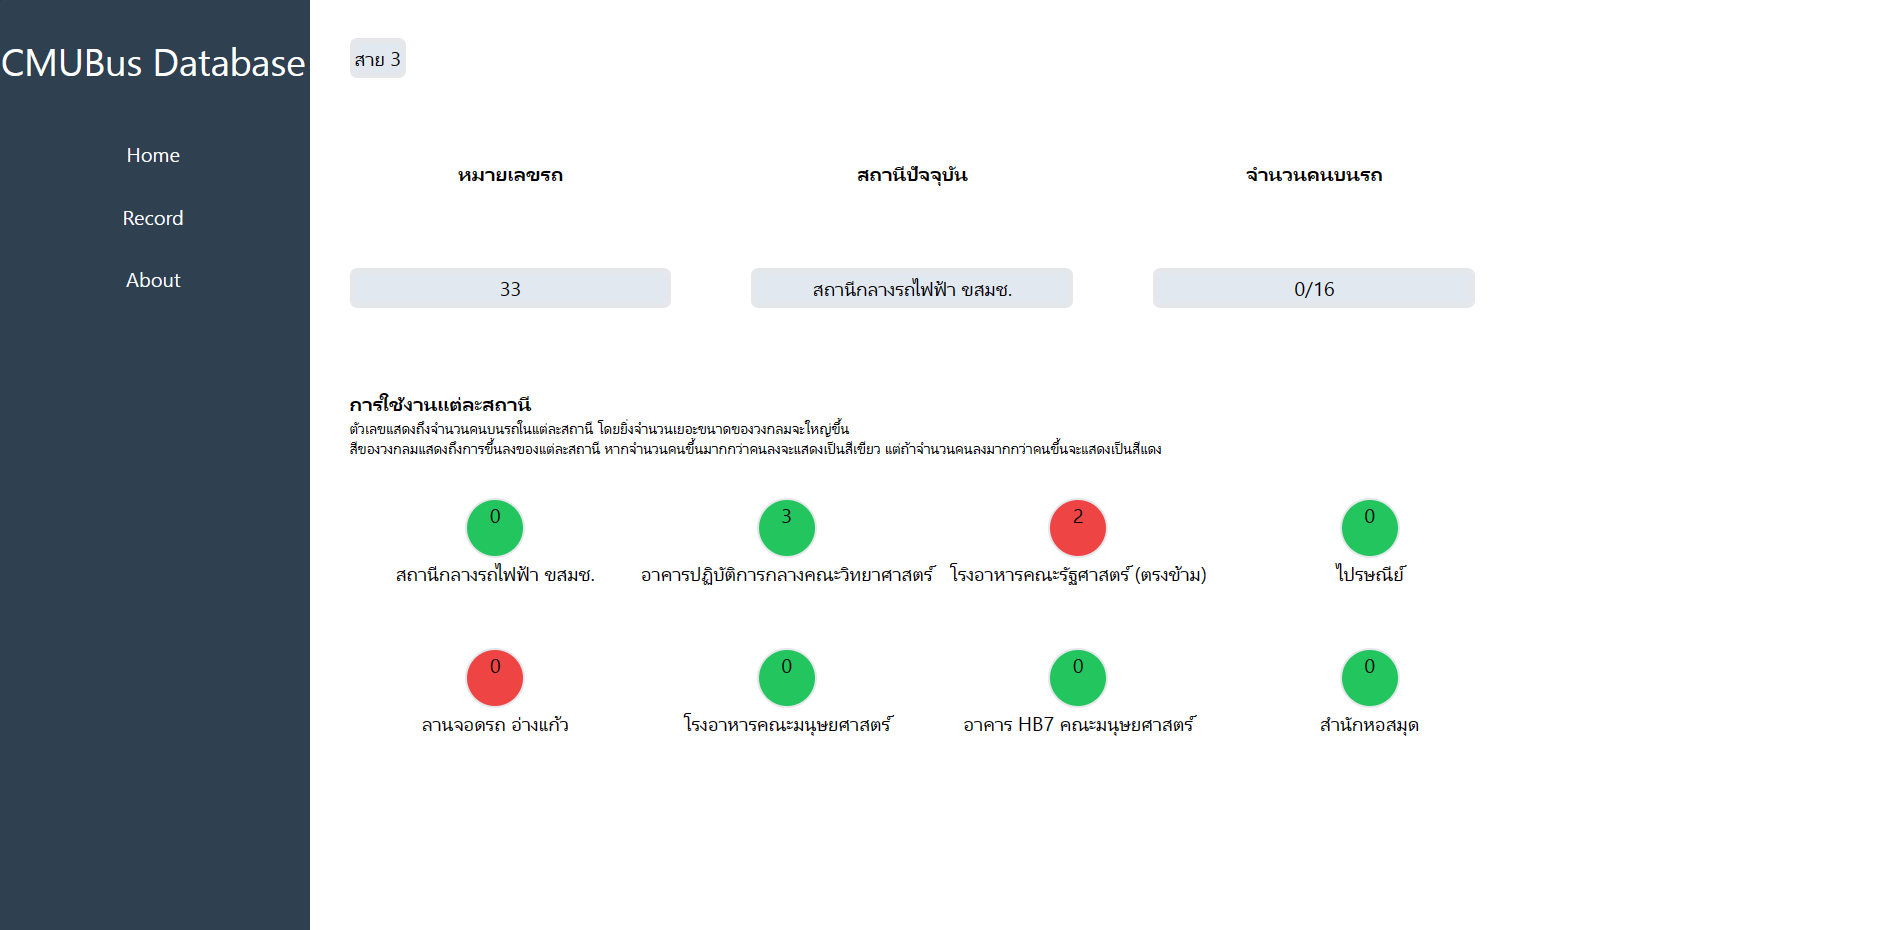
\includegraphics[width=0.75\textwidth]{home.png}
    \end{center}
    \caption{เว็บไซต์หน้า Home}
    \label{fig:home}
  \end{figure}

  \begin{figure}[h!]
    \begin{center}
      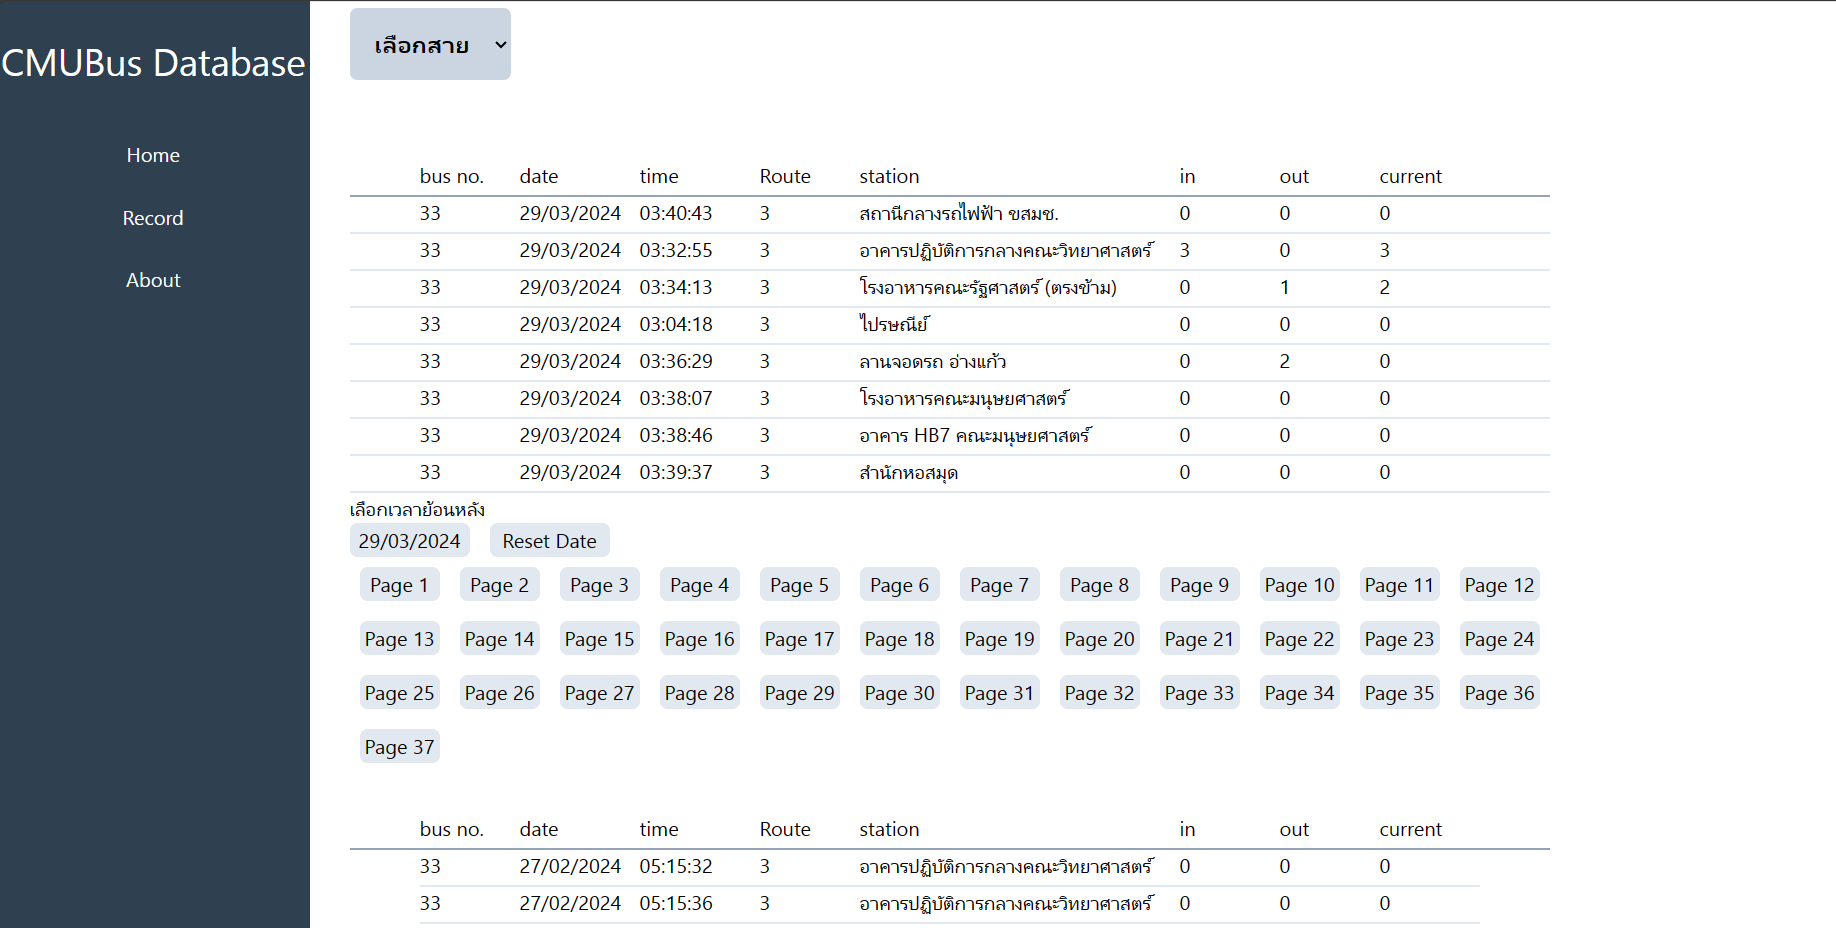
\includegraphics[width=0.75\textwidth]{record.png}
    \end{center}
    \caption{เว็บไซต์หน้า Record}
    \label{fig:record}
  \end{figure}

  \begin{figure}[h!]
    \begin{center}
      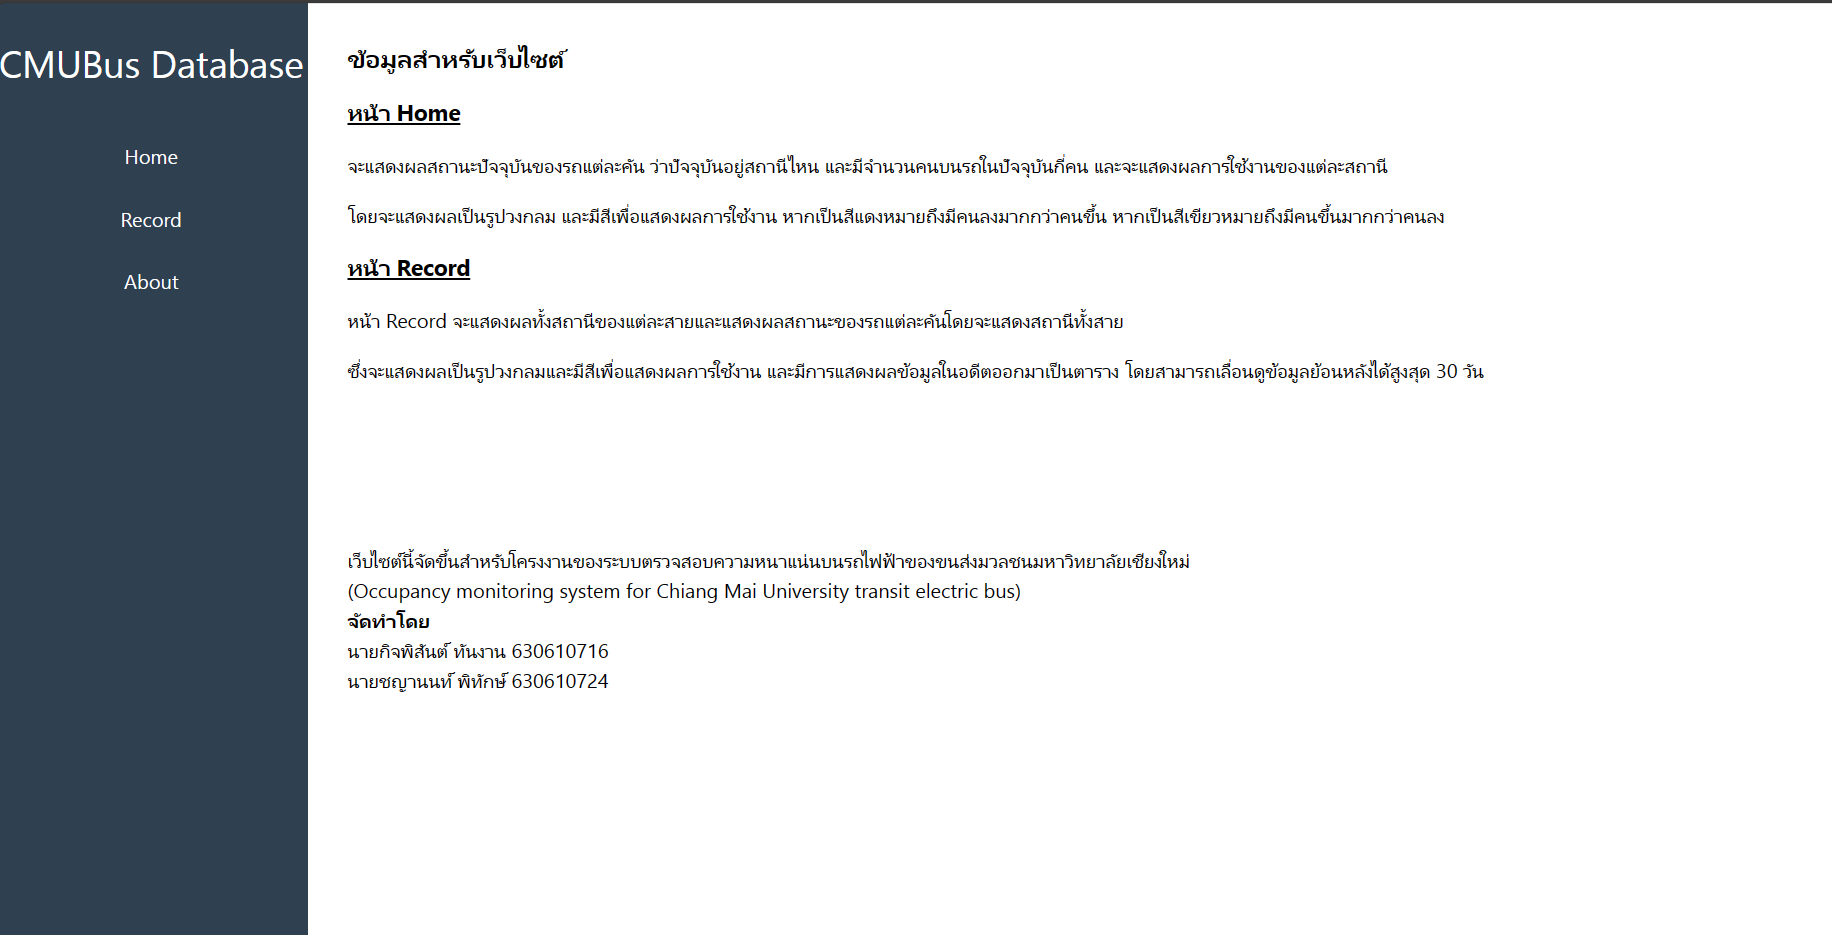
\includegraphics[width=0.75\textwidth]{about.png}
    \end{center}
    \caption{เว็บไซต์หน้า About}
    \label{fig:about}
  \end{figure}